\documentclass{article}
\usepackage[utf8]{inputenc}

\usepackage{amsmath,amssymb,amsfonts}
\usepackage{listings}
\usepackage{graphicx}

\usepackage{hyperref}
\hypersetup{
    colorlinks=true,
    linkcolor=blue,
}

\title{Computational Geometry}
\author{Alvan Caleb Arulandu \& Sameer Gabbita }
\date{March 2021}

\begin{document}

\maketitle

\section{Introduction}
Geometry is a branch of math concerning points, lines, and higher dimensional surfaces. It is also a common topic in higher divisions of competitive programming contests including but not limited to USACO, ICPC, and Codeforces. This lecture will cover common computational geometry algorithms as well as basic mathematical tricks to assist you in solving harder problems.

\section{Vectors}
A vector is a geometric object with a magnitude and direction that can be represented as a list of components in each dimension for most intensive purposes.
$$\vec{x}=\mathbf{x}=[x_{1},x_{2},\cdots,x_{n}]\in \mathbb{R}^{n}$$
Vectors can be represented by drawing an arrow from an arbitrary starting point (say the origin) to an end point given by the components of the vector. 

\subsection{Elementary Operations}
\subsubsection{Scalar Multiplication}
To multiply a vector $\vec{x}\in\mathbb{R}^{n}$ by scalar $s\in\mathbb{R}$, simply multiply each component by the scalar:
$$s\vec{x}=\vec{y}=[y_{1},y_{2},\cdots,y_{n}]:y_{i}=s\cdot a_{i}\, \forall \, 1\leq i\leq n$$

\subsubsection{Addition}
To add to vectors $\vec{a},\vec{b}$, simply add up each component:
$$\vec{a}+\vec{b}=\vec{c}=[c_{1},c_{2},\cdots,c_{n}] : c_{i}=a_{i}+b_{i}\, \forall\, 1\leq i\leq n$$
To subtract vectors, simply add the $(-1)\vec{b}$ which can be calculated with scalar multiplication.

\subsubsection{Magnitude}
The magnitude of $\vec{v}$ can be interpreted as the length of the "arrow" from the start to end point. Using a generalized Pythagorean Theorem we have,
$$|\vec{v}|=v=\sqrt{\sum_{i=1}^{n}v_{i}^{2}}$$
Unit vectors are vectors with magnitude $1$. These can often make computations easier where magnitude is irrelevant.
$$\hat{v}=\frac{\vec{v}}{|\vec{v}|}$$
In 3D space $\hat{i},\hat{j},\hat{k}$ represent the $3$ unit vectors lying on the axes $x,y,z$ respectively. Note that every vector can be written as a sum of it's components times a unit vector along each component axis.

\subsubsection{Dot Product}
There are two types of vector multiplication, one of which is known as the dot product. The dot product computes a sum of element-wise multiplications of two vectors yielding a scalar.
$$\vec{a}\cdot\vec{b}=\sum_{i=1}^{n}a_{i}b_{i}$$
The vector dot product also has a nice geometric interpretation when it comes to vector projection:
$$\vec{a}\cdot\vec{b}=|a||b|\cos\theta$$
Here we say that $\vec{b}$ is projected onto $\vec{a}$. As shown by the above relationship with $\cos$ the vector dot product yields useful information about the angle between two vectors in an $O(n)$ computation.

\subsubsection{Cross Product}
The second type of vector multiplication is known as the cross product and is a method of multiplying two vectors to yield a third orthogonal vector. We can represent the vector cross product as a matrix determinant:
$$\vec{a}\times\vec{b}=|\vec{a}||\vec{b}|\sin\theta\cdot\hat{n}$$
Note that $\hat{n}$ is the unit vector orthogonal to $\vec{a},\vec{b}$.
For $n=3$ the following notational trick can be used for computation:
$$=\det\left(
\begin{bmatrix}
\hat{x_{1}} & \hat{x_{2}} & \hat{x_{n}} \\
a_{1}       & a_{2}       & a_{3} \\
b_{1}       & b_{2}       & b_{3}
\end{bmatrix}
\right)$$
The cross product also has a ton of neat relationships and applications.
$$|\vec{a}\times\vec{b}|=|\vec{a}||\vec{b}|\sin\theta$$

\subsubsection{Uses}
Vector properties are frequently used in distance computations between various objects (commonly seen in multi-variable calculus). Additionally, the multiplicative properties of vectors can be exploited to determine if line segments are perpendicular. 

\section{Coordinate Systems}
Most readers are well aware of Cartesian coordinates $(x,y)$. However, in some cases other coordinate systems like polar can be used to solve problems. Instead of relying on rectangular position, polar coordinates represent points with a radius $r$ and a phase/angle $\theta$; $(r,\theta)$. In this system,
$$r^{2}=x^{2}+y^{2}$$
$$\tan\left(\frac{y}{x}\right)=\theta$$
Please note that this implies that the same point can be represented in infinite ways in polar coordinates. This only applies to two dimensions but there are similar systems available for three dimensions. Cylindrical coordinates are similar to polar coordinates with an added $z=z$ equality; $(r,\theta,z)$. Spherical coordinates introduce a third angular parameter $\phi$ which is the angle from the radius to the $z$ axis; $(\rho,\theta,\phi)$.

\section{Sweep Line Algorithms}
Sweep-line algorithms are a set of algorithms that follow a similar idea regarding, you guessed it - a sweeping line! These algorithms imagine sweeping a line across a plane stopping at points that intersect or are in close proximity to the line. A certain operation is then done on these points such that a complete solution is available by the time the line crosses the entire plane.

\subsection{Line Segment Intersection}
The line segment intersection problem consists of detection and calculation. One task is to determine if a set of line segments have an intersection. The other is to determine all intersections of the line segments.

\subsubsection{Two Segments}
The "algorithm" for two segments is fairly simple and amounts to a plethora of if statements checking orientation cases for detection and Cramer's rule for calculation.

\subsubsection{Bentley-Ottmann Algorithm}
However, for $n>2$ line segments, is harder. A naive approach (testing every pair) takes $O(n^{2})$. But, using this sweep line algorithm allows us to calculate a list of intersection points from a set of line segments in $O((n+k)\log n)$ time where $n$ is the number of line segments and $k$ is the number of intersections. Note that worst case, $k=\frac{n(n-1)}{2}$.

\subsubsection{Shamos-Hoey Algorithm}
As a side-note, this algorithm applies binary search trees to this problem yielding $O(n\log n)$ complexity to detect line segment intersections.

\section{Convex Hull}
Convex Hull is an algorithm that can find the smallest convex polygon that contains all given points (aka the convex hull) for 2D or 3D points and are bounded by the upper bound theorem for higher dimensions. Naively, finding the convex hull takes $O(n^3)$ time where we can iterate through all possible line segments, and add it to the convex hull if all the other points are to its left.
\subsection{Graham Scan}
\begin{lstlisting}[language=python]
def graham_scan(points):
    st = []
    p0 = point with smallest y-coordinate
    sort_ccw(points)
    st = [points[0], points[1]]
    for i in range(2, len(points)):
        while len(stack) > 2 and points[i] is right of st[-1] and st[-2]:
            st.pop()
        st.push(points[i])
        
\end{lstlisting}

\subsection{Andrew's Algorithm}
\begin{lstlisting}[language=python]
def andrews_algo(points):
    sort_by_x_coordinate(points)
    upper = []
    lower = []
    for point in points:
        while direction() == left:
            upper.remove(second_to_last_point)
        upper.append(point)
    for point in points:
        while direction() == right:
            lower.remove(second_to_last_point)
        lower.append(point)
    convex_hull = merge()
    return convex_hull
\end{lstlisting}

\begin{figure}[h!]
\centering
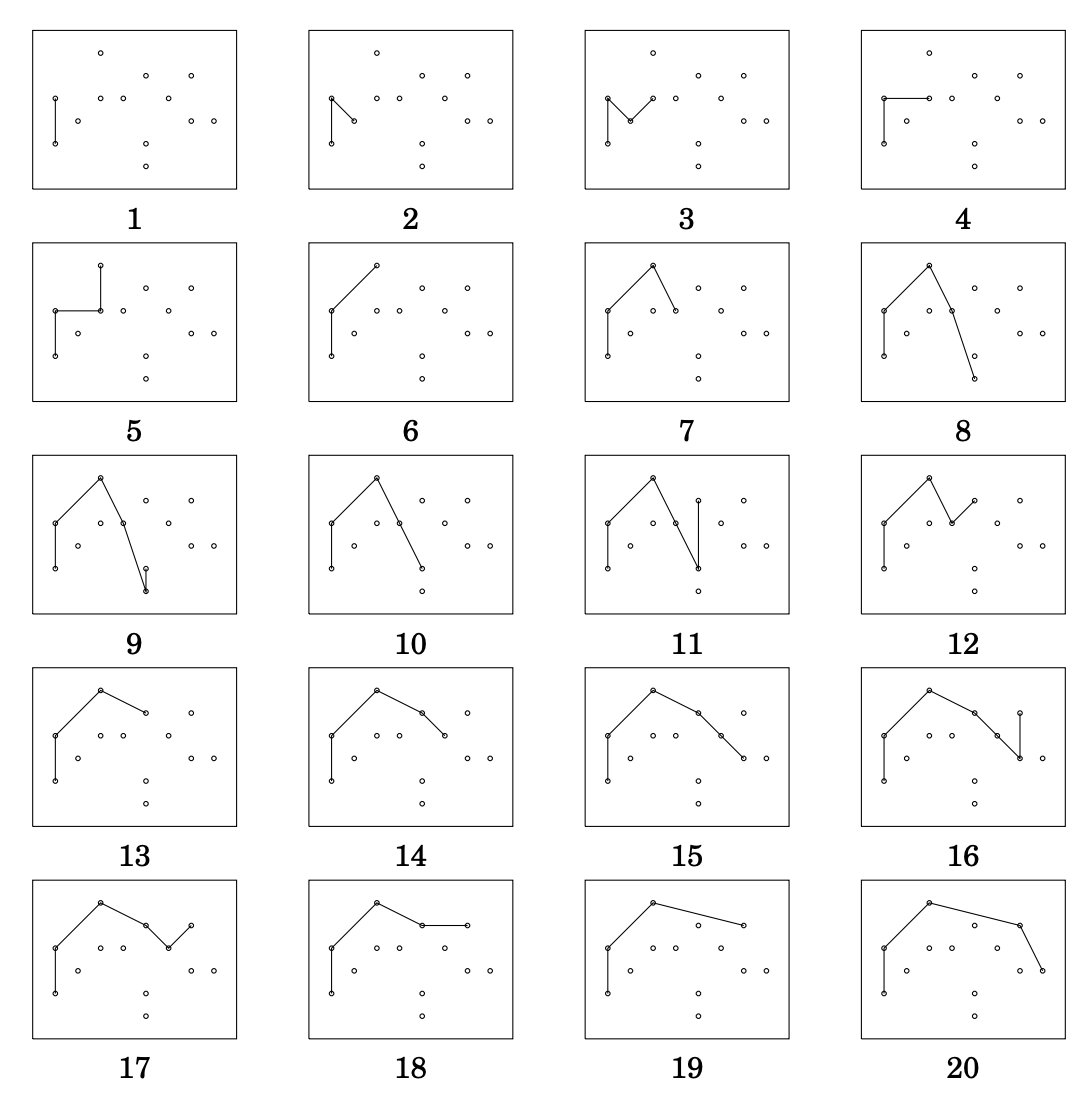
\includegraphics[scale=.5]{Andrew's Scan.png}
\caption{Andrew's Scan (From CPH)}
\label{fig:Convex Hull}
\end{figure}

\section{Distances}
\subsection{Point-Plane}
$$D=|\hat{n}\cdot(\vec{p}-\vec{q})|$$
where $\hat{n}$ is the unit normal vector of the plane, $\vec{p}$ is the point, and $\vec{q}$ is an arbitrary point on the plane.
\subsection{Point-Point}
$$D=|\vec{a}-\vec{b}|$$
where $\vec{a},\vec{b}$ are vectors to the points of interest.
\subsection{Point-Line}
$$D=|\hat{n}\cdot(\vec{p}-\vec{q})|$$
where $\hat{n}$ is the unit normal vector from the line, $\vec{p}$ is the point, and $\vec{q}$ is an arbitrary point on the line.
\subsection{Plane-Plane}
If the planes are parallel, pick an arbitrary point on one and use Point-Plane. Otherwise, the planes must intersect so the distance is $0$.
\subsection{Line-Line}
If the lines are parallel, pick an arbitrary point on one of the lines and use Point-Line. Otherwise, find the distance between the two parallel planes each containing one of the lines.
\subsection{Plane-Line}
If the line is parallel to the plane, then use Point-Plane with an arbitrary point on the line. Otherwise, they must intersect so the distance is $0$.

\subsection{Shoelace Theorem}
\subsubsection{Statement}
Suppose polygon $P$ has vertices $(a_{1},b_{1}),(a_{2},b_{2}),\cdots,(a_{n},b_{n})$ in clockwise order. Then the area $A$ of $P$ is
$$A=\frac{1}{2}|\sum_{i=1}^{n}(x_{i+1}+x_{i})(y_{i+1}-y_{i})|$$
$$=\frac{1}{2}|(a_{1}b_{2}+a_{2}b_{3}+\cdots+a_{n}b_{1})-(b_{1}a_{2}+b_{2}a_{3}+\cdots+b_{n}a_{1})|$$

\subsubsection{Algorithm}
This method works by dividing up the polygon into many triangles formed from 2 vertices of the polygon and an origin $O$. We can then sum the areas of those individual triangles to find the total area of a polygon. To find the area of these individual triangles, we can use the cross-product, which gives the area of a parallelogram, and divide it by 2 to find the area of the triangle. As a result, this algorithm runs in $O(n)$ time where $n$ is the number of points in the polygon.

\subsection{Pick's Theorem}
Pick's theorem can be used for lattice-point polygons as states,
$$\text{Area}=a + \frac{b}{2} - 1$$
where $a$ is the number of lattice points strictly inside a polygon and $b$ is the number of lattice points that are on the edges of a polygon.

\subsection{Cramer's Rule}
Cramer's rule is a way to analytically solve a system of equations using the determinant of a matrix. Given the following system of equations
$$\begin{array}{lcl} a_1x + b_1y + c_1z = d_1 \\ a_2x + b_2y + c_2z = d_2 \\ a_3x + b_3y + c_3z = d_3\end{array}$$

we can solve the system of equations where $x = D_x/D$, $y = D_y/D$, $z = D_z/D$ given that $D \neq 0$ where 
$$
D=\det\left(
\begin{bmatrix}
a_{1} & b_{1} & c_{1} \\
a_{2} & b_{2} & c_{2} \\
a_{3} & b_{3} & c_{3}
\end{bmatrix}
\right)
$$

$$
D_x=\det\left(
\begin{bmatrix}
d_{1} & b_{1} & c_{1} \\
d_{2} & b_{2} & c_{2} \\
d_{3} & b_{3} & c_{3}
\end{bmatrix}
\right)
$$

$$
D_y=\det\left(
\begin{bmatrix}
a_{1} & d_{1} & c_{1} \\
a_{2} & d_{2} & c_{2} \\
a_{3} & d_{3} & c_{3}
\end{bmatrix}
\right)
$$
$$
D_z=\det\left(
\begin{bmatrix}
a_{1} & b_{1} & d_{1} \\
a_{2} & b_{2} & d_{2} \\
a_{3} & b_{3} & d_{3}
\end{bmatrix}
\right)
$$

\section{Miscellaneous}
This section contains a list of miscellaneous topics that you may/may not encounter in competitive programming problems but is included for sake of completeness and the reader's own interest.

\subsection{Upper Bound Theorem}
The theorem states that cyclic polytopes (polytopes formed as a convex hull around a rational normal curve where $n>d$) have the largest possible number of faces among all convex polytopes with a given dimension and number of vertices. Note that $n$ is the number of points and $d$ is the dimension of the space.

\subsection{Area of a Triangle}
$$
[\triangle ABC]=\frac{bh}{2}=\frac{ab\sin C^{\circ}}{2}=\frac{|\vec{u}\times\vec{v}|}{2}
=\sqrt{s(s-a)(s-b)(s-c)}=rs=\frac{abc}{4R}
$$
\subsection{Approximations / Expansions}
$$\sin\theta=\sum_{k=0}^{\infty}\frac{(-1)^{k}\theta^{2k+1}}{(2k+1)!}$$
$$\cos\theta=\sum_{k=0}^{\infty}\frac{(-1)^{k}\theta^{2k}}{(2k)!}$$

\section{Problems}
\subsection{Practice}
\begin{itemize}
    \item \href{http://usaco.org/index.php?page=viewproblem2&cpid=943}{Cow Steeplechase II}
    \item \href{https://codeforces.com/problemset/problem/1299/C}{Water Balance}
    \item \href{https://cses.fi/problemset/}{CSES Geometry Problems}
    \item \href{https://open.kattis.com/problems/imperfectgps}{Imperfect GPS}
    \item \href{https://open.kattis.com/problems/polygonarea}{Polygon Area}
    \item \href{https://codeforces.com/contest/598/problem/F}{Cut Length}
\end{itemize}
\subsection{Custom: Hurdles}
\subsubsection{Problem}
Gleb is running the "free-meter" hurdles. There are $N$ hurdles given as points $(x_{i},y_{i})$ in the Cartesian plane such that $|x|,|y|<10^{9}$ and no two points $(x_{1},y_{1}),(x_{2},y_{2})$ are co-linear with the origin $(0,0)$. Gleb starts at $(1,0)$ and must cross each hurdle exactly once in any particular order before returning to the starting point to finish the race. There is no hurdle at the starting point. If Gleb runs at $\pi e$ meters per second, what is the floor of the minimum time to finish the race so that Gleb can smoke the competition? 
\subsubsection{Input}
Input starts with one line containing the integer $1<N<10^{8}$. The next $N$ lines contain two comma separated integers $x,y$. Ex:
\begin{lstlisting}
3
1,1
-1,0
0,-1
\end{lstlisting}
\subsection{Output}
Output should consist of one integer, the floor of the minimum time. For this example, the total distance is $1+\sqrt{5}+2\sqrt{2}\approx6.06\rightarrow 6$. Ex:
\begin{lstlisting}
6
\end{lstlisting}

\section{Sources}
\begin{itemize}
    \item \href{https://artofproblemsolving.com/wiki/index.php/Shoelace_Theorem}{Shoelace Theorem (AOPS)}
    \item \href{https://www.youtube.com/watch?v=0KjG8Pg6LGk}{Shoelace Theorem (Mathologer)}
    \item \href{https://artofproblemsolving.com/wiki/index.php/Pick's_Theorem}{Pick's Theorem (AOPS)}
    
    \item \href{https://usaco.guide/CPH.pdf#page=288}{Andrew's Algorithm (USACO Guide)}
    \item \href{https://www.cs.ucr.edu/~eldawy/19SCS133/slides/CS133-04-ConvexHull.pdf}{Graham Scan (CS133)}

\end{itemize}
\end{document}
